\documentclass[]{scrartcl}

\usepackage{graphicx}
\usepackage{amsmath}

%opening
\title{ASSIGNMENT 1}
\author{Esteve Tarrago Sanchis}

\begin{document}

\maketitle

\abstract



\section{Simulation Results}
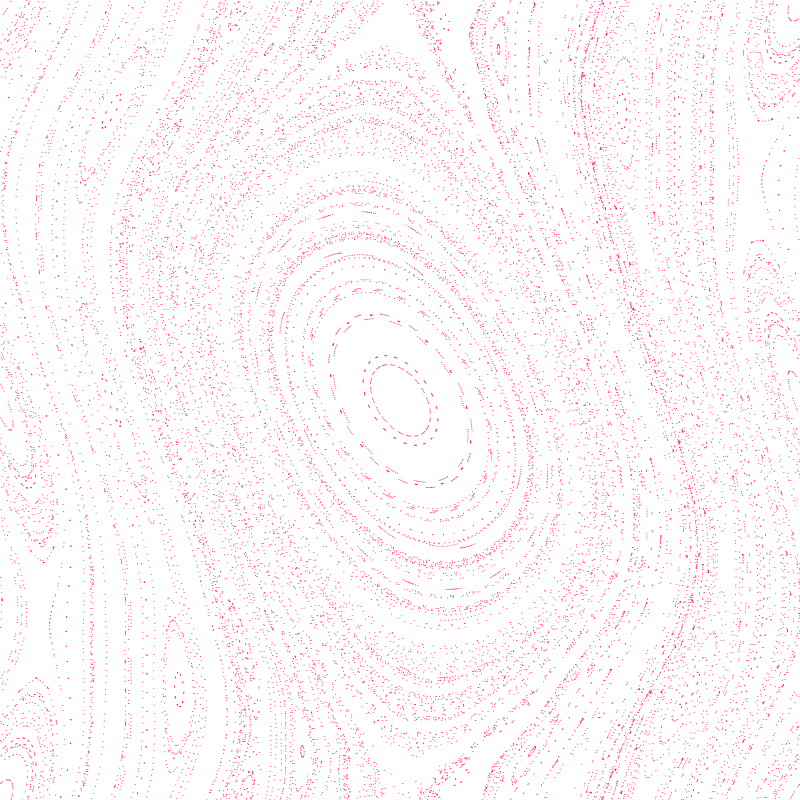
\includegraphics[width=\linewidth]{orbit.png}

The image on top shows the orbit generated by 250 random seeds in the domain with 100 iterations of the map.
\section{Exact 2-periodic points}
In order to find the exact solution we will proceed analytically.
Being F the dynamical map:

$
F(
\begin{bmatrix}
x \\
y \\
\end{bmatrix}) =  \begin{bmatrix}
x + a * sin(x + y) \\
x + y \\
\end{bmatrix}
$

The equation a point has to fulfill to be two periodic is:

$
F(F(
\begin{bmatrix}
	x \\
	y \\
\end{bmatrix})) =  \begin{bmatrix}
x \\
y \\
\end{bmatrix}
$

By substitution:

$
F(
\begin{bmatrix}
x + a * sin(x + y) \\
x + y \\
\end{bmatrix}) =  \begin{bmatrix}
x \\
y \\
\end{bmatrix}
$

And again:

$
\begin{bmatrix}
x + a * sin(x + y) + a * sin(x + a * sin(x + y) + x + y) \\
x + a * sin(x + y) + x + y \\
\end{bmatrix} =  \begin{bmatrix}
x \\
y \\
\end{bmatrix}
$

Using the second row we obtain:

$
a * sin(x + y) = - 2*x
$

By substitution in the first row:

$
- 2*x + a * sin(y) = 0
$

Isolating x:

$
x = a * sin(y)/2
$



We can express the solution as:

$
\begin{bmatrix}
a * sin(y)/2 \\
y \\
\end{bmatrix}
$

(0,0) and (0,$\pi$) are solutions but we discard them cause they are equilibrium points.

One example of 2-periodic point would be (a/2,$\pi$/2).


\section{Approximate 3-periodic points}
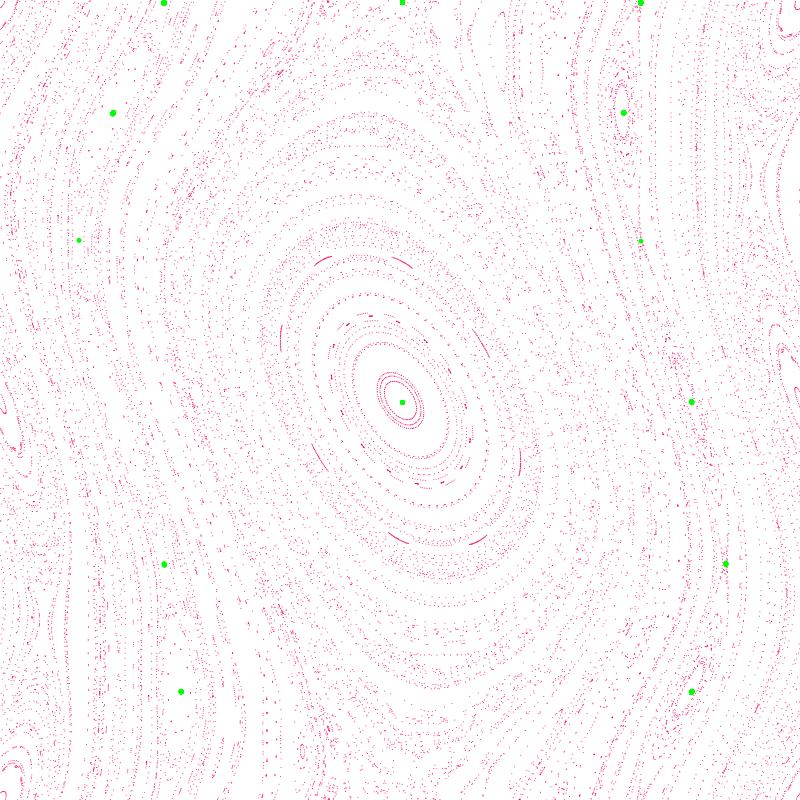
\includegraphics[width=\linewidth]{k3.png}
In green you can see the numerical some numerical solutions obtained for $F^3(X) = X$. You can see we find again equilibrium points also plotted in green.

Some numeric values are:

1.738091841344433, 2.272693953960068,

1.8712855525053995, 3.139591126041121

2.2739822843670643, -2.2704212354909648

\section{Approximate 4-periodic points}
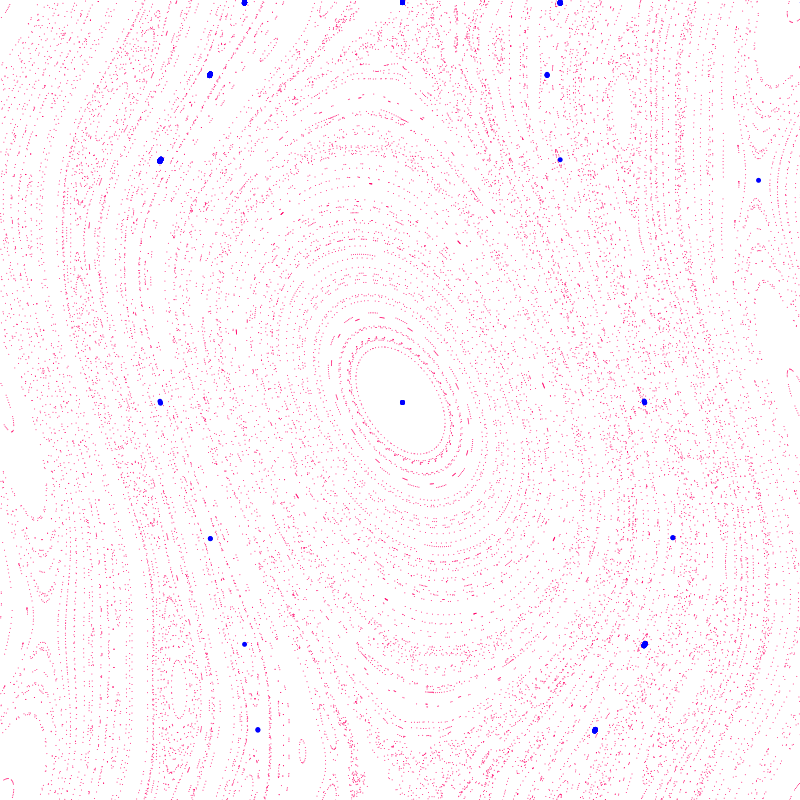
\includegraphics[width=\linewidth]{k4.png}
In blue you can see the numerical some numerical solutions obtained for $F^4(X) = X$. You can see we find again equilibrium points also plotted in blue.

Some numeric values are:

-1.508663922159468, 2.5807669229866903

1.9065899112674964,-1.8934780387244492

1.23878287680494, 3.1394713507992167
\section{Chaos}
There clearly exist Chaos in some regions of the map. We can see this in the regions between two nearby stable equilibrium points. A slight difference in the beginning of the trajectory lead us two completely different orbits.
\section{Invariant curves}
Around the equilibrium points we can see periodic elliptic orbits that define invariant curves. 
\section{Dynamic comments}
Most of points in the system are stable points but not asymptotically stable which generate a lot of periodic orbits in the plot.

Also the fact that the domain is a torus generate two more equilibrium points + periodic orbits.


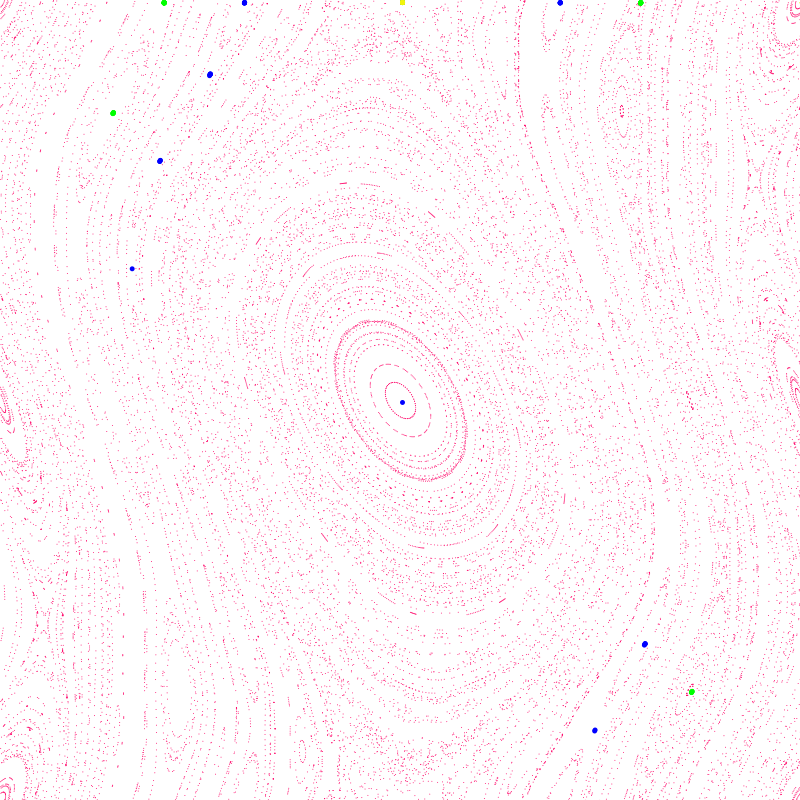
\includegraphics[width=\linewidth]{allk.png}


\end{document}
